\documentclass{beamer}
\usepackage{graphics}
\usepackage{color}
\usepackage{listings}

\xdefinecolor{ay_struct_color}{rgb}{0.09,0.17,0.41}
\xdefinecolor{ay_norm_color}{rgb}{0.3,0.3,0.3}

\setbeamercolor{structure}{fg=ay_struct_color}
\setbeamercolor{ay_norm_color}{fg=ay_norm_color}
\logo{
\includegraphics[width=100px]{logo.jpg}}

\author{Fedor Nikitin}
\title{Statistical analysis of PIFs inversions}

\begin{document}
  \maketitle

  \frame{
    \frametitle{Goal}
    \bf Hypothesis: \rm
    Shorter distance and more adjacent legs $\Rightarrow$ more inversions.

    \vspace{10pt}
    \bf Goal: \rm to support validity of hypothesis with data.
  }

  \frame{
    \frametitle{PIFs inversion measure}
    \begin{itemize}
      \item Analyze inversion corrected PIFs before modified by users
      \item Current inversion algorithm produce long sequences of same values when PIFs inverted
      \item Longer sequence $\Rightarrow$ more inversions
      \item One year data analyzed 
      \item Exclude legs with length $>=$ 3000 km
    \end{itemize}

    \vspace{10pt}
    \bf Measure $pi$: \rm number of distinct PIFs.

    \vspace{10pt}
    Greater $pi$ $\Rightarrow$ less inversions and vice versa.
  }

  \frame{
    \frametitle{Features}
    \begin{itemize}
      \item $avg_i$ --- sample mean of $pi$ for leg $i$ 
      \item $adjnum_i$ is number of adjacent legs to leg $i$
      \item $dist_i$ is distance to fly over leg $i$
    \end{itemize}
  }

  \frame{
    \frametitle{pi vs adjnum}
    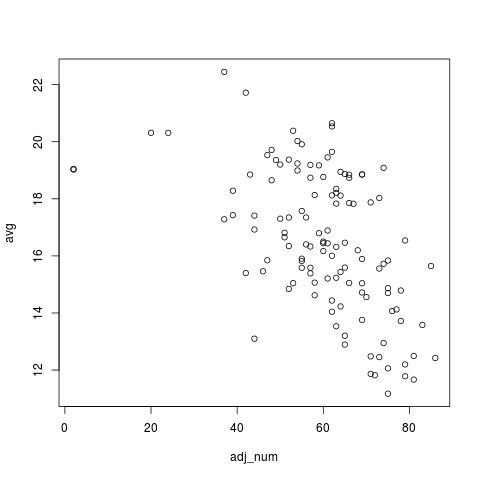
\includegraphics[width=300px,height=200px]{adj_num_avg.png}
  }

  \frame{
    \frametitle{pi vs log(dist)}
    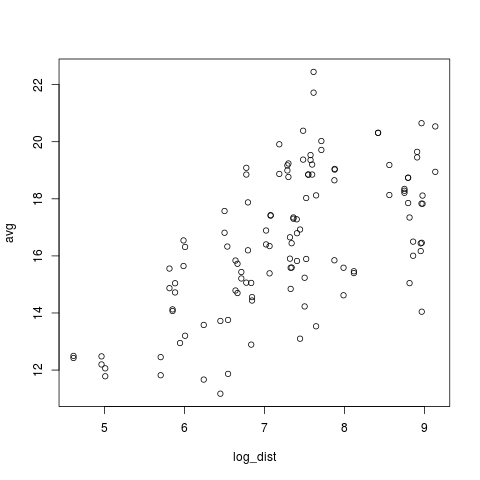
\includegraphics[width=300px,height=200px]{log_dist_avg.png}
  }

  \frame{
    \frametitle{Regression}
    Model:
    $$
    pi = a_0 + a_1 * log( dist ) + a_2 * adjnum
    $$
    Fit:
    $$
    pi = 8.2 + 1.5 * log( dist ) - 0.05 * adjnum
    $$
    Quality:
    $$
    R^2 = 0.48
    $$
  }

  \frame{
    \frametitle{Residuals}
    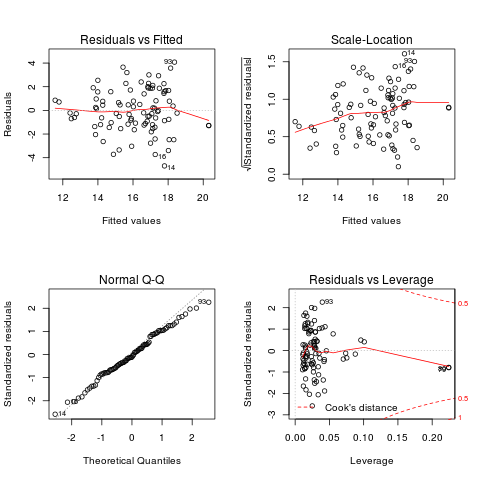
\includegraphics[width=300px,height=200px]{res.png}
  }

  \frame{
    \frametitle{Conclusions}
    \begin{itemize}
      \item Longer leg $\Rightarrow$ less inversions
      \item Greater number of adjacent legs $\Rightarrow$ more inversions
    \end{itemize} 
  }

\end{document}




